\documentclass{article}\usepackage[]{graphicx}\usepackage[]{color}
%% maxwidth is the original width if it is less than linewidth
%% otherwise use linewidth (to make sure the graphics do not exceed the margin)
\makeatletter
\def\maxwidth{ %
  \ifdim\Gin@nat@width>\linewidth
    \linewidth
  \else
    \Gin@nat@width
  \fi
}
\makeatother

\definecolor{fgcolor}{rgb}{0.345, 0.345, 0.345}
\newcommand{\hlnum}[1]{\textcolor[rgb]{0.686,0.059,0.569}{#1}}%
\newcommand{\hlstr}[1]{\textcolor[rgb]{0.192,0.494,0.8}{#1}}%
\newcommand{\hlcom}[1]{\textcolor[rgb]{0.678,0.584,0.686}{\textit{#1}}}%
\newcommand{\hlopt}[1]{\textcolor[rgb]{0,0,0}{#1}}%
\newcommand{\hlstd}[1]{\textcolor[rgb]{0.345,0.345,0.345}{#1}}%
\newcommand{\hlkwa}[1]{\textcolor[rgb]{0.161,0.373,0.58}{\textbf{#1}}}%
\newcommand{\hlkwb}[1]{\textcolor[rgb]{0.69,0.353,0.396}{#1}}%
\newcommand{\hlkwc}[1]{\textcolor[rgb]{0.333,0.667,0.333}{#1}}%
\newcommand{\hlkwd}[1]{\textcolor[rgb]{0.737,0.353,0.396}{\textbf{#1}}}%
\let\hlipl\hlkwb

\usepackage{framed}
\makeatletter
\newenvironment{kframe}{%
 \def\at@end@of@kframe{}%
 \ifinner\ifhmode%
  \def\at@end@of@kframe{\end{minipage}}%
  \begin{minipage}{\columnwidth}%
 \fi\fi%
 \def\FrameCommand##1{\hskip\@totalleftmargin \hskip-\fboxsep
 \colorbox{shadecolor}{##1}\hskip-\fboxsep
     % There is no \\@totalrightmargin, so:
     \hskip-\linewidth \hskip-\@totalleftmargin \hskip\columnwidth}%
 \MakeFramed {\advance\hsize-\width
   \@totalleftmargin\z@ \linewidth\hsize
   \@setminipage}}%
 {\par\unskip\endMakeFramed%
 \at@end@of@kframe}
\makeatother

\definecolor{shadecolor}{rgb}{.97, .97, .97}
\definecolor{messagecolor}{rgb}{0, 0, 0}
\definecolor{warningcolor}{rgb}{1, 0, 1}
\definecolor{errorcolor}{rgb}{1, 0, 0}
\newenvironment{knitrout}{}{} % an empty environment to be redefined in TeX

\usepackage{alltt}

\usepackage[margin=1in]{geometry}
\usepackage{parskip}
\IfFileExists{upquote.sty}{\usepackage{upquote}}{}
\begin{document}

{\Large \bf Warm-up Exercise}

April 3, 2017

\bigskip

Student-to-faculty ratio data collected from random samples of public and private four-year colleges:

\begin{minipage}[c]{0.4\textwidth}
\begin{center}
\begin{tabular}{lrrr}
  \hline
type & mean & SD & n \\ 
  \hline
private & 13.84 & 7.28 &  85 \\ 
  public & 17.60 & 4.57 &  57 \\ 
   \hline
\end{tabular}
\end{center}
\end{minipage}
\begin{minipage}[c]{0.6\textwidth}
\begin{center}
% \includegraphics[width=0.8\textwidth]{ratio/ratio_box.pdf}




\begin{knitrout}
\definecolor{shadecolor}{rgb}{0.969, 0.969, 0.969}\color{fgcolor}
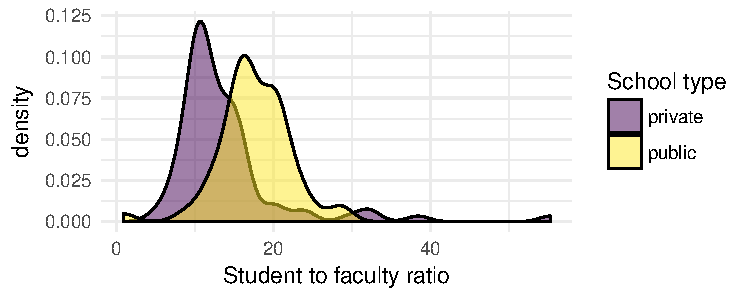
\includegraphics[width=\maxwidth]{figure/unnamed-chunk-1-1} 

\end{knitrout}
\end{center}
\end{minipage}


\begin{enumerate}

\item We would like to test if there is a \emph{difference} between the average student-to-faculty ratio between public and private four-year colleges using a randomization test. What are the hypotheses?

\vspace{.5in}

\item How is the reference distribution (i.e. the permutation distribution) created?

\vspace{1in}

% \item Fill in the blanks below for the appropriate set up for this test:
% 
% \begin{doublespace}
% We write the student-to-faculty ratio of each public and private college in this sample on a total of \rule{2cm}{0.5pt} index cards. Then, we shuffle these cards and split them into two groups: one group of size \rule{2cm}{0.5pt} representing public colleges, and another group of size \rule{2cm}{0.5pt} representing private colleges. We calculate the difference between the average student-to-faculty ratios in the public and private colleges ($\bar{x}_{public} - \bar{x}_{private}$) and record this value. We repeat this many times to build a randomization distribution, which should be centered at \rule{2cm}{0.5pt} . Lastly, we calculate the p-value as the proportion of simulations where the simulated differences in means are \rule{5cm}{0.5pt}.
% \end{doublespace}


\item The histogram below is created using 9,999 resamples. What is the p-value? To help you answer this the smallest and largest 10 differences in means are displayed below.

% \begin{center}
% \includegraphics[width=0.8\textwidth]{ratio/rand_dist_dot.pdf}
% \end{center}

\begin{knitrout}
\definecolor{shadecolor}{rgb}{0.969, 0.969, 0.969}\color{fgcolor}
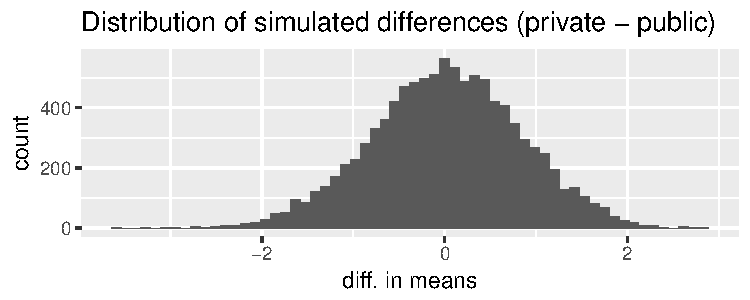
\includegraphics[width=\maxwidth]{figure/unnamed-chunk-2-1} 

\end{knitrout}

\begin{knitrout}\scriptsize
\definecolor{shadecolor}{rgb}{0.969, 0.969, 0.969}\color{fgcolor}\begin{kframe}
\begin{verbatim}
##               [,1]      [,2]      [,3]      [,4]      [,5]      [,6]      [,7]      [,8]      [,9]     [,10]
## smallest -3.581598 -3.303189 -3.028894 -2.898691 -2.775187 -2.753880 -2.703525 -2.692080 -2.644764 -2.584326
## largest   2.333110  2.354737  2.378760  2.419961  2.560588  2.570464  2.600881  2.656252  2.745697  2.845808
\end{verbatim}
\end{kframe}
\end{knitrout}


\vspace{.25in}


\item Based on the p-value, do these data provide convincing evidence to suggest that the student-to-faculty ratio in public four-year colleges is different than that of private four-year colleges.


\end{enumerate}


\end{document}
